\newpage
\section{Visualization}

The Orthogonal Vector Visualization System provides comprehensive visualization options for the generated vectors. This section describes the visualization techniques used by the system, including the enhanced axis representation and scaling features.

\subsection{3D Visualization}

The 3D visualization shows the vectors in three-dimensional space. It uses Matplotlib's 3D plotting capabilities to create a 3D plot with the following features:

\begin{itemize}
    \item The origin point is shown as a red dot for high visibility.
    \item The vectors can be shown as arrows from the origin point or just as endpoints.
    \item Each vector is assigned a different color for easy identification, using a colormap for multiple vectors.
    \item The plot includes a legend identifying each vector.
    \item The plot includes labels for the X, Y, and Z axes.
    \item Color-coded axis lines (X: red, Y: green, Z: blue) with coordinate labels.
    \item Small tick marks along each axis for better spatial reference.
    \item Data-driven axis scaling that focuses on the actual data points.
    \item Equal aspect ratio to ensure accurate spatial representation.
    \item The plot includes a title, which can be customized.
\end{itemize}

\subsubsection{Enhanced Axis Representation}

The enhanced axis representation is implemented through the \texttt{setup\_enhanced\_3d\_axes} function, which provides the following features:

\begin{itemize}
    \item \textbf{Color-coded axes:} The X, Y, and Z axes are color-coded (red, green, and blue by default) for easy identification.
    \item \textbf{Coordinate labels:} The axes include coordinate labels at regular intervals, showing the numerical values along each axis.
    \item \textbf{Data-driven scaling:} The axis limits are determined based on the actual data points, with a configurable buffer factor to ensure all points are visible.
    \item \textbf{Equal aspect ratio:} The plot maintains an equal aspect ratio to ensure accurate spatial representation of the vectors.
    \item \textbf{Customizable appearance:} The appearance of the axes can be customized through configuration parameters.
\end{itemize}

\subsubsection{Manual Axis Enhancement Approach}

In addition to the \texttt{setup\_enhanced\_3d\_axes} function, the system also supports a manual approach to axis enhancement, as demonstrated in the \texttt{perfect\_circle\_distance\_range.py} example script. This approach provides fine-grained control over the visualization and includes the following features:

\begin{itemize}
    \item \textbf{Explicit axis lines:} The X, Y, and Z axes are explicitly drawn as lines with custom colors (red, green, and blue).
    \item \textbf{Custom coordinate markers:} Coordinate markers are placed at integer intervals along each axis, with small tick marks for better readability.
    \item \textbf{Axis labels:} Large, colored labels (X, Y, Z) are placed at the end of each axis.
    \item \textbf{Data-driven scaling:} The axis limits are calculated based on the actual data range, with a buffer factor for better visibility.
    \item \textbf{Equal aspect ratio:} The plot uses a box aspect ratio of [1, 1, 1] to ensure accurate spatial representation.
\end{itemize}

This manual approach is particularly useful for customized visualizations where precise control over the appearance of the axes is required. The code for this approach is included in the appendix as part of the \texttt{perfect\_circle\_distance\_range.py} script.

The 3D visualization provides a complete view of the vectors in three-dimensional space, allowing for a better understanding of their spatial relationships.

\begin{figure}[H]
    \centering
    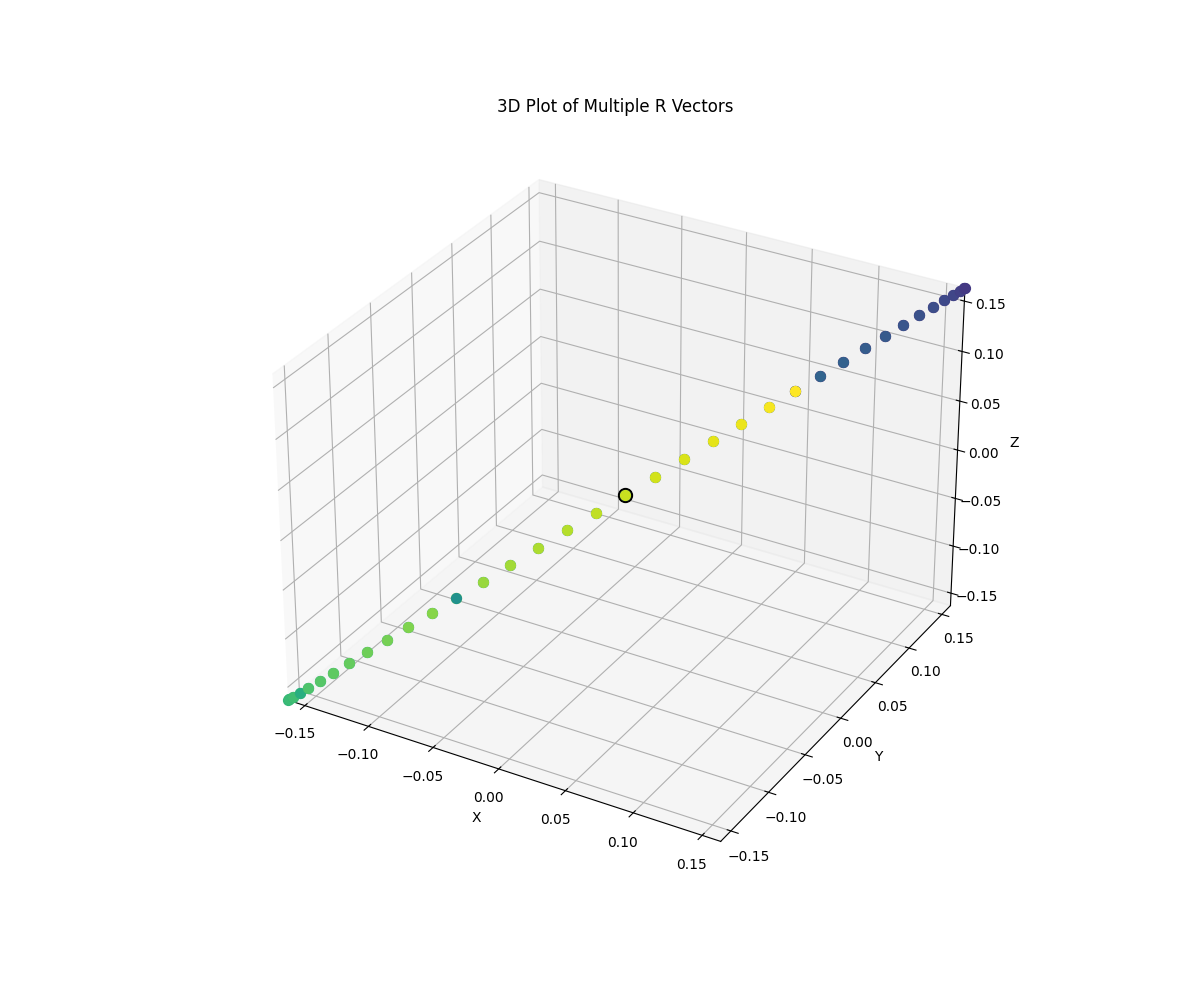
\includegraphics[width=0.8\textwidth]{figures/orthogonal_3d.png}
    \caption{Example of 3D visualization of orthogonal vectors}
    \label{fig:vis_3d_plot}
\end{figure}

\subsection{2D Projections}

The 2D visualization shows projections of the vectors onto various planes. It creates four subplots showing the following projections:

\begin{itemize}
    \item XY Plane: Shows the projection of the vectors onto the XY plane (Z=0).
    \item XZ Plane: Shows the projection of the vectors onto the XZ plane (Y=0).
    \item YZ Plane: Shows the projection of the vectors onto the YZ plane (X=0).
    \item Origin Plane: Shows the projection of the vectors onto the plane perpendicular to the vector from the global origin to the specified origin point.
\end{itemize}

Each subplot includes the following features:

\begin{itemize}
    \item The origin point is shown as a black dot.
    \item The vectors can be shown as arrows from the origin point or just as endpoints.
    \item Each vector is assigned a different color for easy identification, using a colormap for multiple vectors.
    \item The subplot includes a legend identifying each vector.
    \item The subplot includes labels for the axes.
    \item Color-coded axis lines with coordinate labels when enhanced visualization is enabled.
    \item Data-driven scaling that focuses on the actual data points.
    \item Equal aspect ratio to ensure accurate spatial representation.
    \item The subplot includes a title indicating the plane of projection.
\end{itemize}

\subsubsection{Orthogonal Plane Projection}

When enhanced visualization is enabled, the 2D visualization includes a projection onto the plane orthogonal to the x=y=z line. This projection is particularly useful for visualizing the perfect orthogonal circle, as it shows the circle as a perfect circle in this projection. The projection is implemented using the basis vectors [1, -1/2, -1/2] and [0, -1/2, 1/2], which form an orthogonal basis for the plane perpendicular to the [1, 1, 1] direction.

The 2D projections provide different perspectives on the vectors, allowing for a better understanding of their projections onto different planes.

\begin{figure}[H]
    \centering
    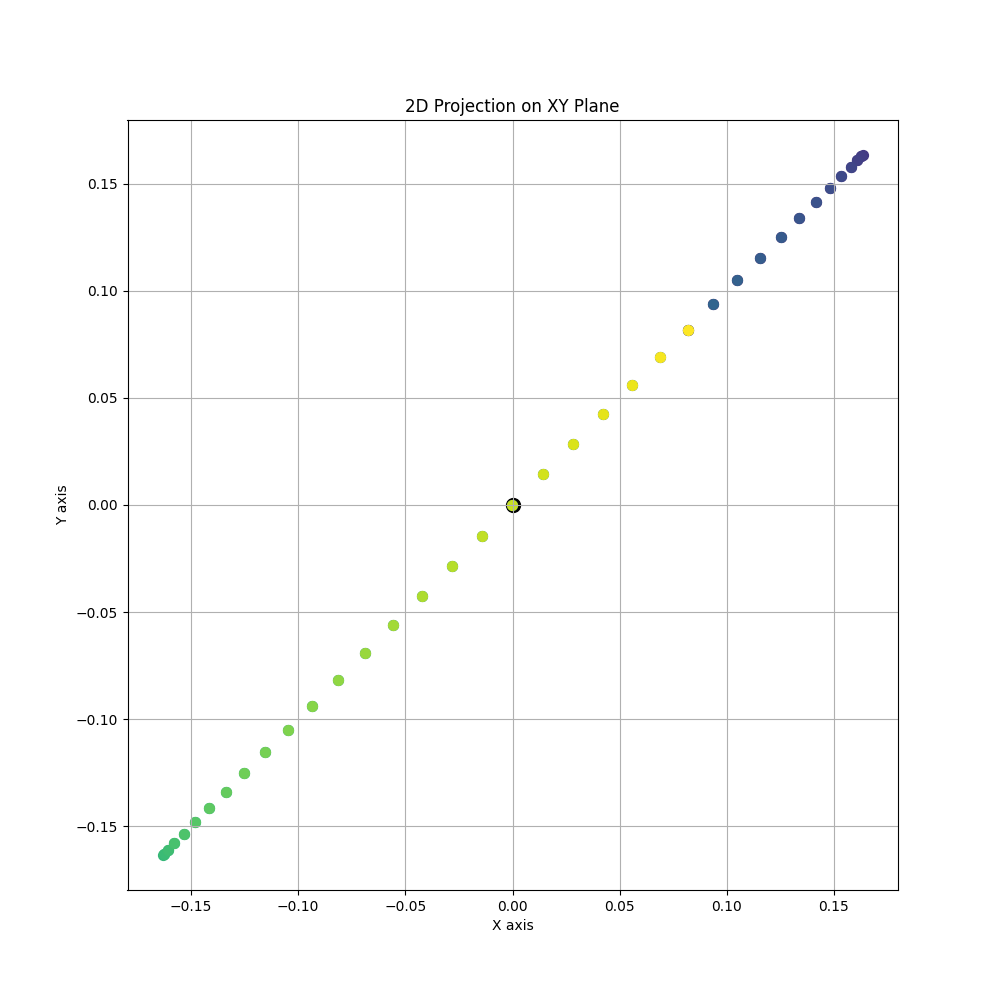
\includegraphics[width=0.45\textwidth]{figures/orthogonal_xy.png}
    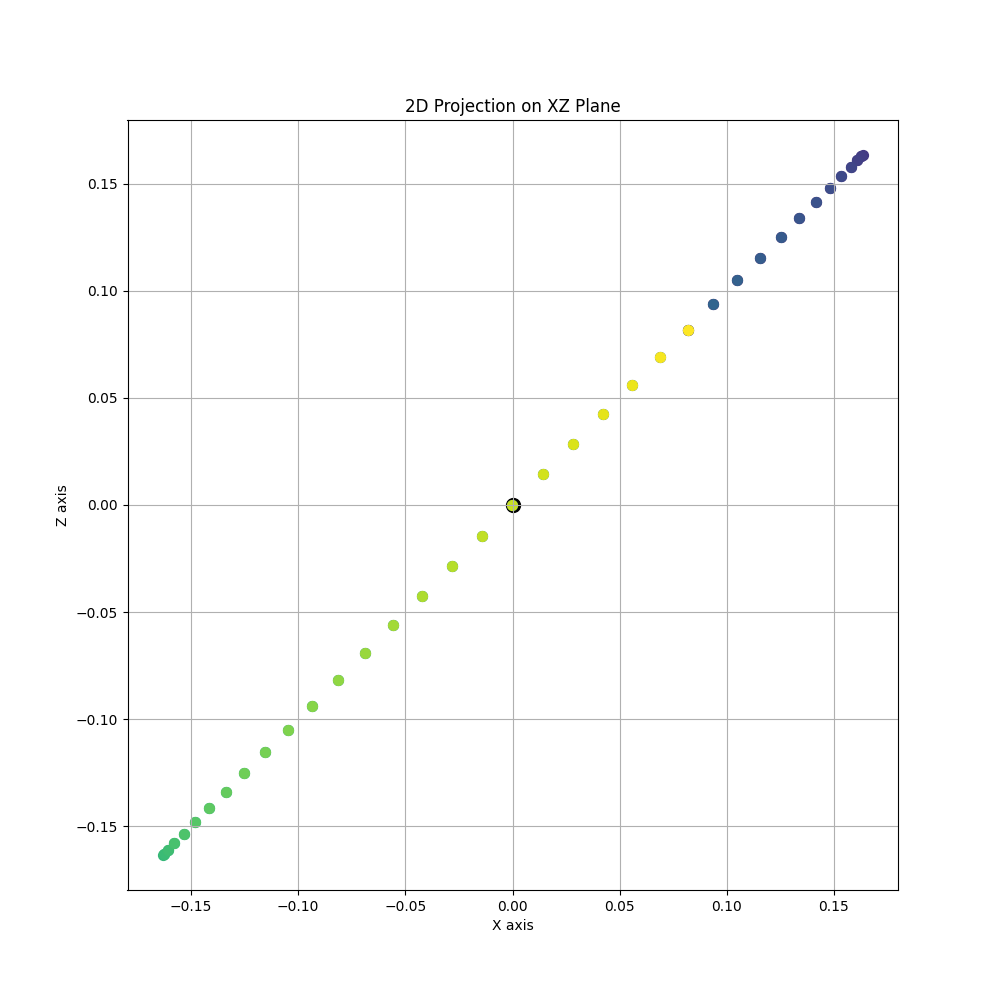
\includegraphics[width=0.45\textwidth]{figures/orthogonal_xz.png}
    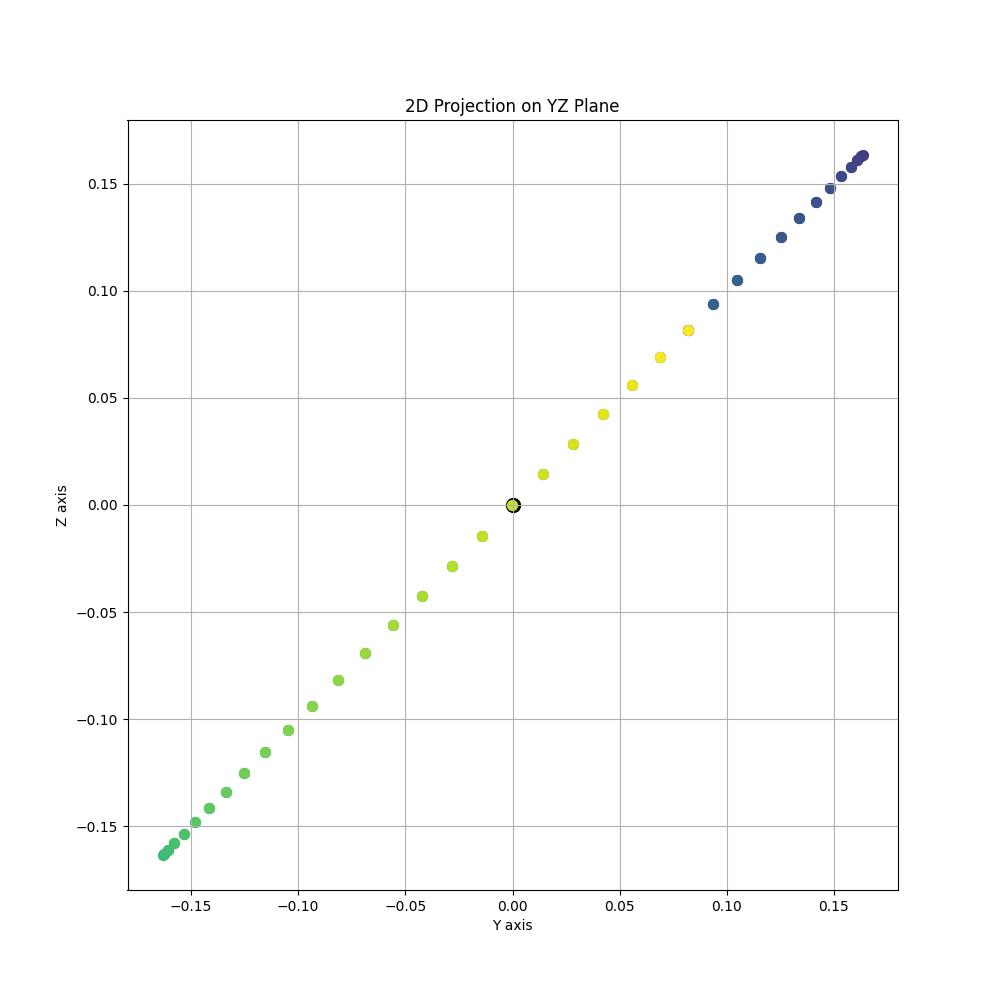
\includegraphics[width=0.45\textwidth]{figures/orthogonal_yz.png}
    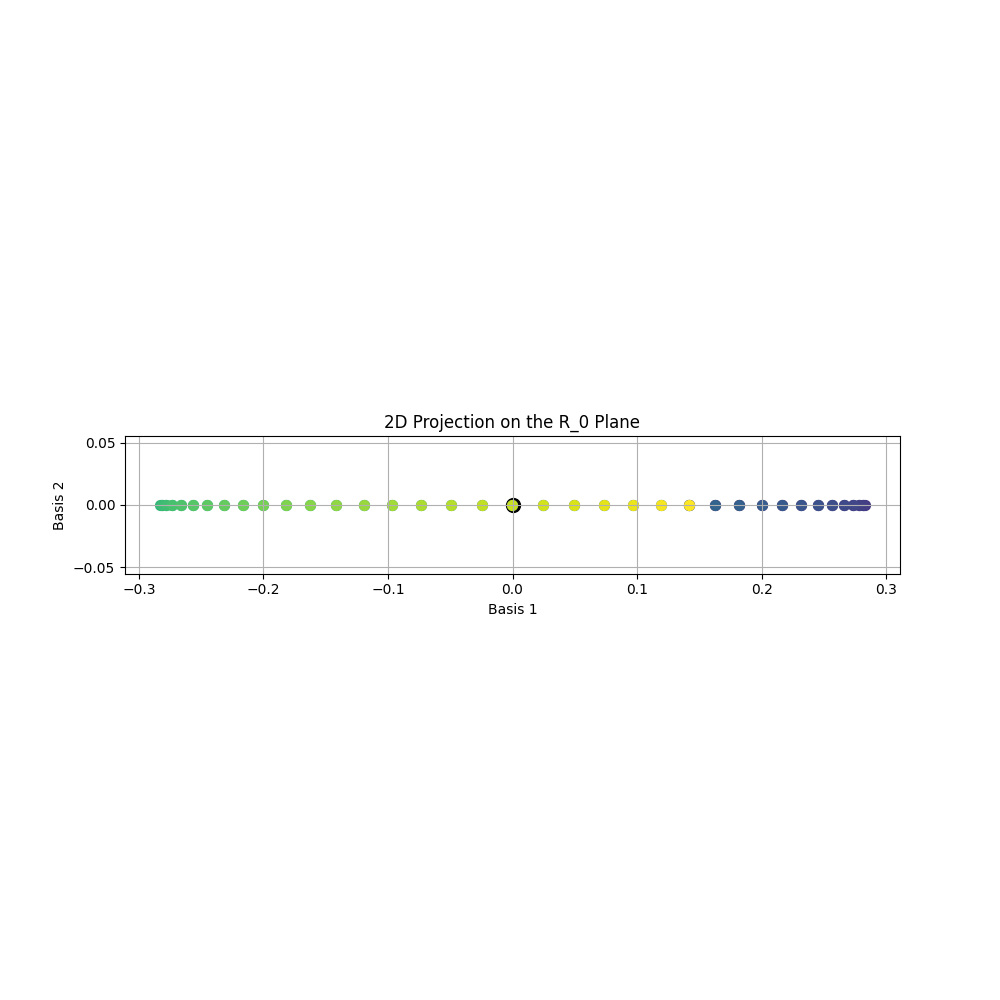
\includegraphics[width=0.45\textwidth]{figures/orthogonal_r0.png}
    \caption{Example of 2D projections of orthogonal vectors}
    \label{fig:vis_2d_projections}
\end{figure}

\subsection{Endpoints-only Plotting}

The system provides an endpoints-only plotting option that only shows the endpoints of vectors, not the arrows. This is particularly useful for visualizing patterns formed by multiple vectors, such as circle or sphere-like patterns.

\begin{itemize}
    \item In 3D visualization, the endpoints are shown as colored dots.
    \item In 2D projections, the endpoints are shown as colored dots in each projection plane.
    \item The endpoints-only option can be enabled using the --endpoints command-line option.
\end{itemize}

This option provides a clearer visualization of point patterns by removing the arrows, which can clutter the plot when there are many vectors.

\begin{figure}[H]
    \centering
    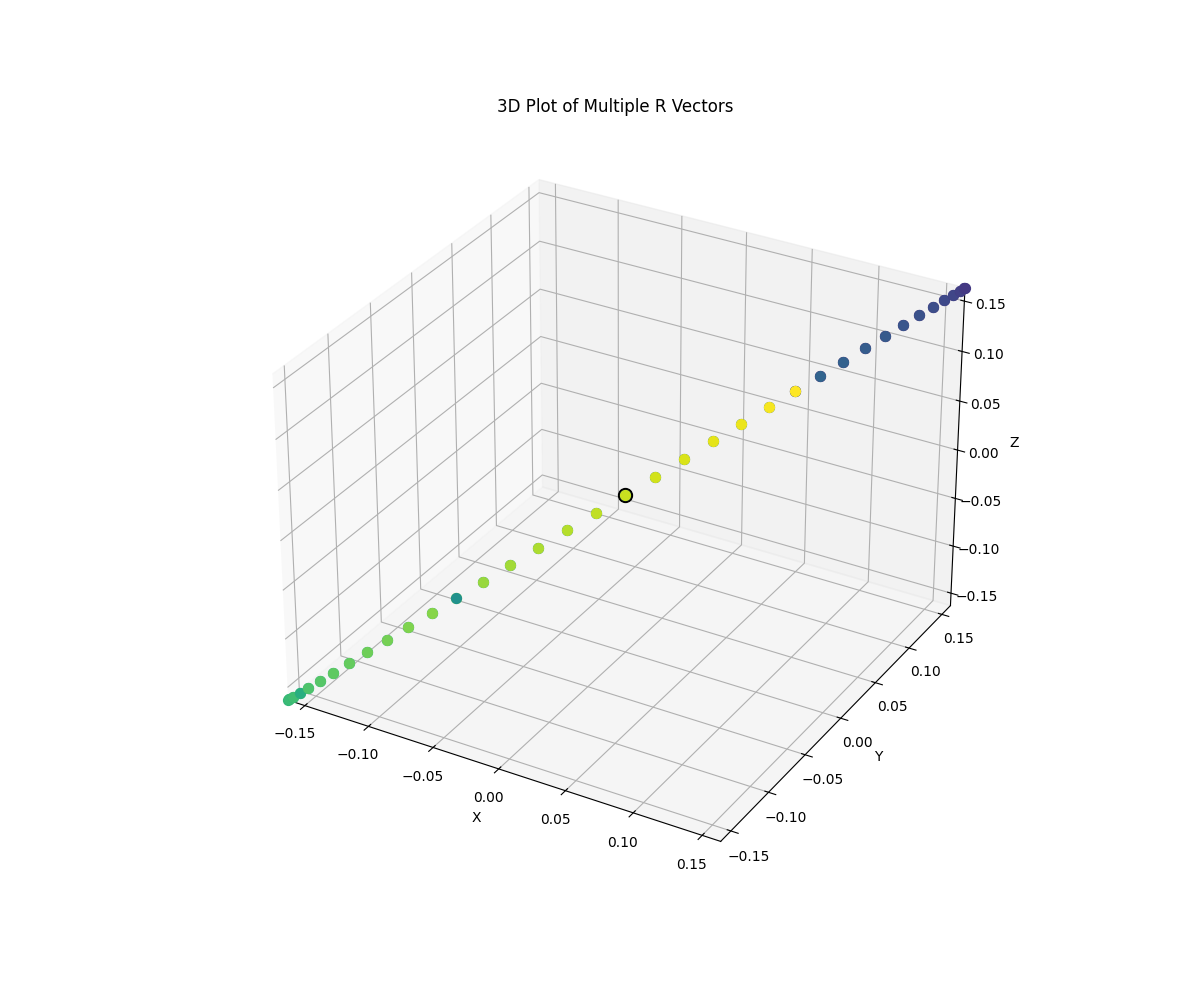
\includegraphics[width=0.8\textwidth]{figures/circle_3d.png}
    \caption{Example of endpoints-only visualization (orthogonal vector circle)}
    \label{fig:vis_endpoints_only}
\end{figure}

\subsection{Multiple Vector Visualization}

The system supports visualizing multiple vectors in a single plot, with the following features:

\begin{itemize}
    \item Multiple vectors can be generated by specifying ranges for the distance and angle parameters.
    \item Each vector is assigned a color from a colormap for easy identification.
    \item The plot includes a legend identifying each vector by its parameters.
    \item The endpoints-only option can be used to visualize the pattern formed by the endpoints of multiple vectors.
\end{itemize}

This capability is particularly useful for exploring the effects of varying parameters on the resulting vectors and for generating complex patterns such as circles and spheres.

\subsection{Circle Examples Visualization}

The system includes example scripts demonstrating different approaches to generating and visualizing circle and sphere-like patterns:

\begin{itemize}
    \item \texttt{example\_circle.py}: Generates points using orthogonal vector formulas, creating a sphere-like pattern.
    \item \texttt{example\_circle\_xy.py}: Creates a traditional circle in the XY plane.
    \item \texttt{example\_orthogonal\_circle.py}: Similar to the first example but with improved visualization.
\end{itemize}

These examples generate points at regular angular intervals and plot only the endpoints of the vectors, providing a clear visualization of the resulting patterns.

\begin{figure}[H]
    \centering
    \begin{minipage}{0.48\textwidth}
        \centering
        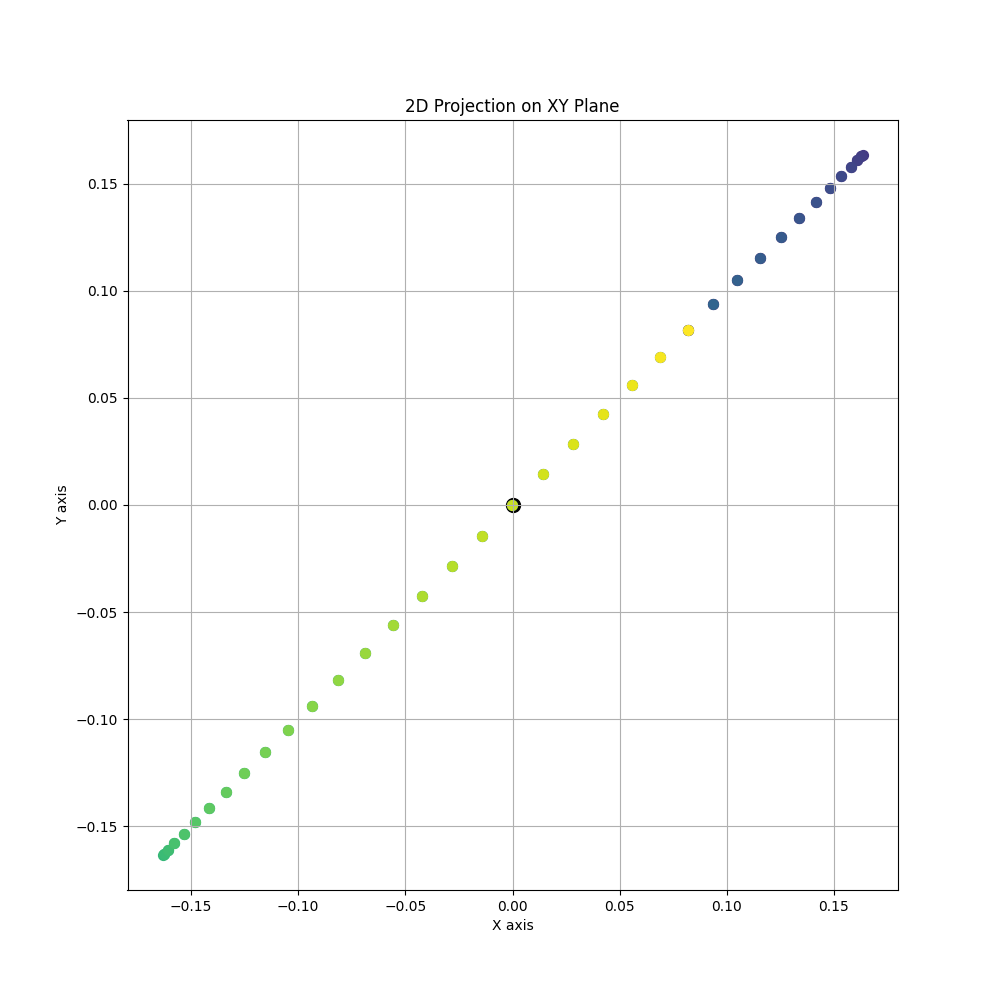
\includegraphics[width=\textwidth]{figures/circle_xy.png}
        \caption{XY projection of orthogonal vector circle}
        \label{fig:vis_circle_xy}
    \end{minipage}\hfill
    \begin{minipage}{0.48\textwidth}
        \centering
        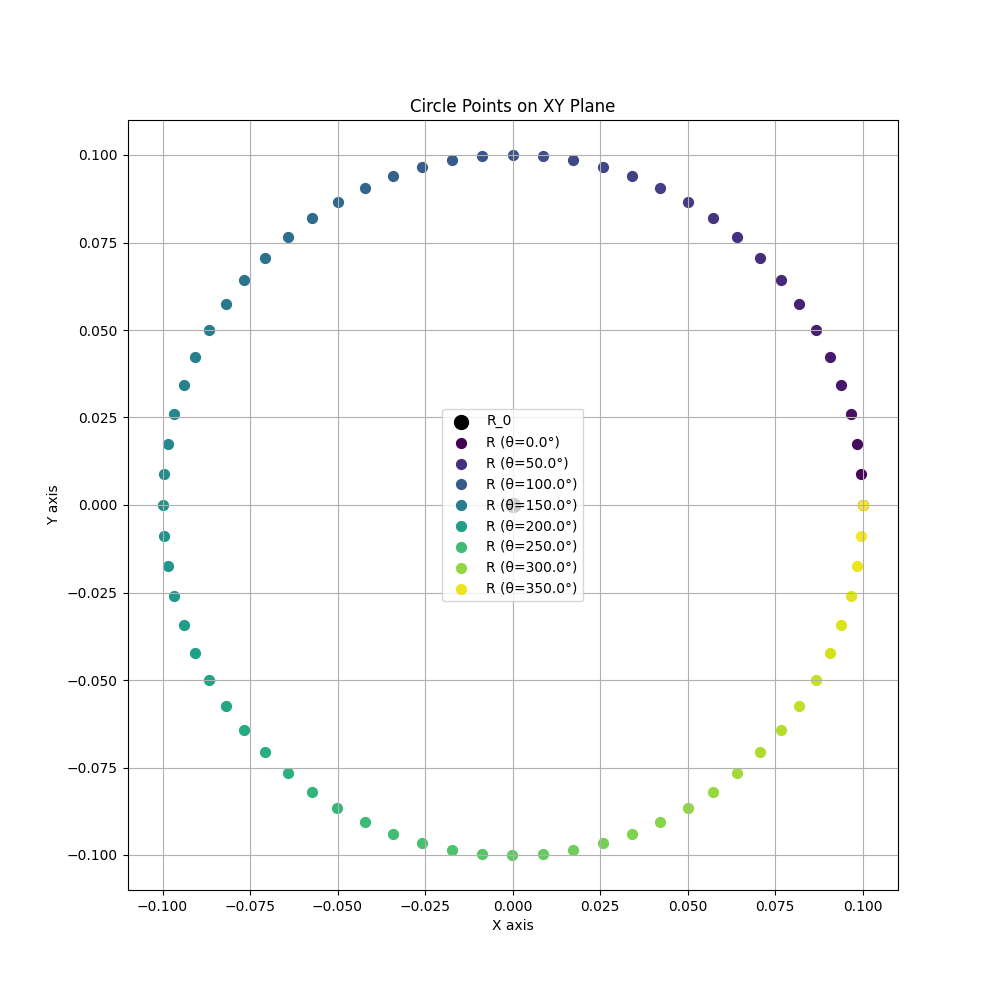
\includegraphics[width=\textwidth]{figures/xy_circle.png}
        \caption{Traditional circle in XY plane}
        \label{fig:vis_xy_circle}
    \end{minipage}
\end{figure}

\begin{figure}[H]
    \centering
    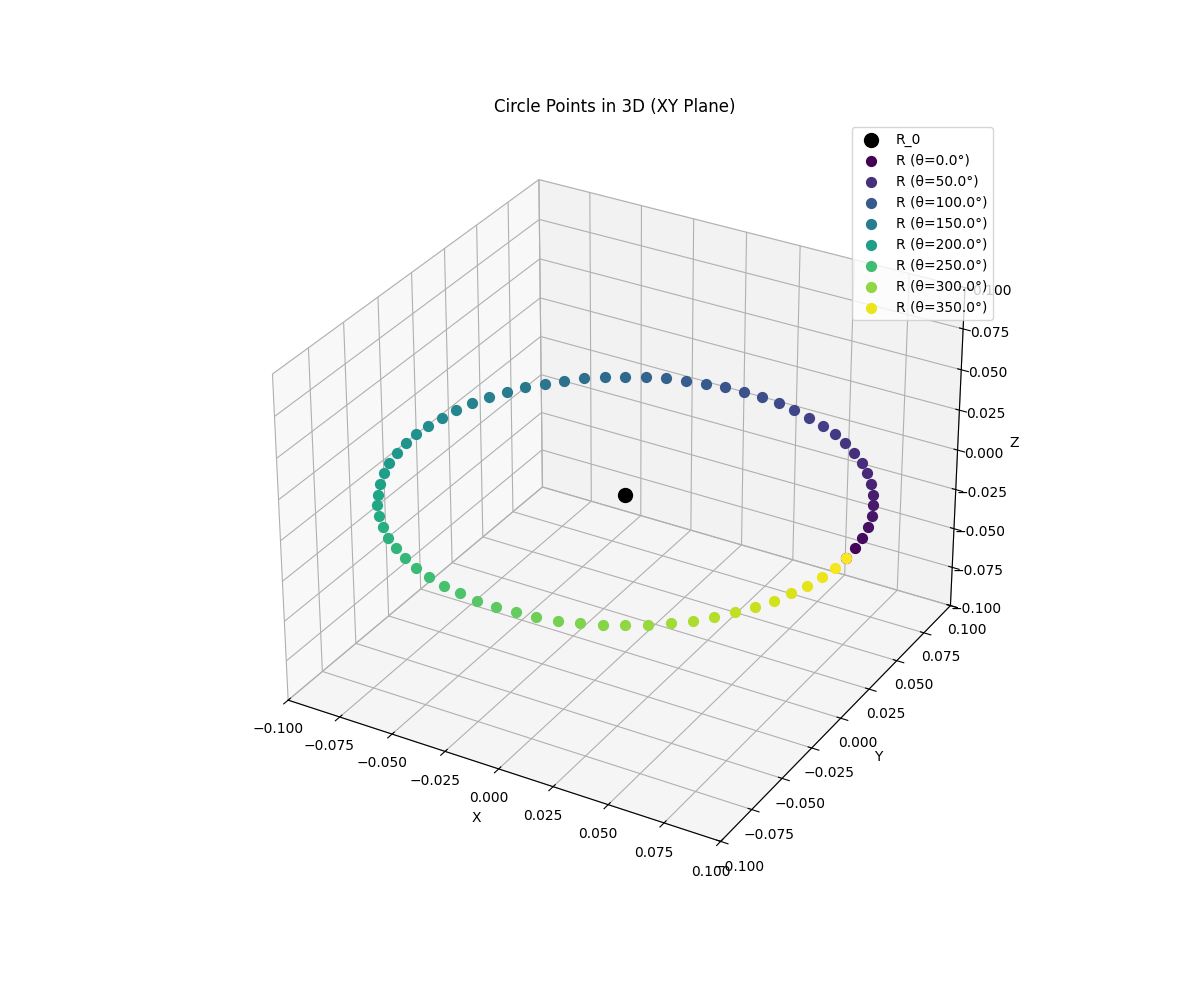
\includegraphics[width=0.8\textwidth]{figures/3d_xy_circle.png}
    \caption{3D visualization of traditional XY circle}
    \label{fig:vis_3d_xy_circle}
\end{figure}

\subsection{Enhanced Axis Representation}

The visualization system includes enhanced axis representation features for better spatial understanding:

\begin{itemize}
    \item \textbf{Color-coded Axes}: The X, Y, and Z axes are color-coded (X: red, Y: green, Z: blue) for easy identification.
    \item \textbf{Coordinate Labels}: Integer coordinate values are displayed along each axis, color-matched to the axis color.
    \item \textbf{Tick Marks}: Small tick marks are added along each axis for better spatial reference.
    \item \textbf{Axis Scaling}: The axis limits are dynamically adjusted based on the actual data points, with a small buffer for better visibility.
    \item \textbf{Equal Aspect Ratio}: The 3D plots maintain an equal aspect ratio for accurate spatial representation.
\end{itemize}

These enhancements significantly improve the visual representation of the orthogonal vectors, making it easier to understand their spatial relationships and properties.

\subsection{Implementation Details}

The visualization functions use Matplotlib to create the plots. The 3D visualization uses Matplotlib's \texttt{Axes3D} class, while the 2D visualizations use regular Matplotlib axes.

The vectors are plotted using Matplotlib's \texttt{quiver} function, which creates arrows from a starting point to an ending point. The origin point is plotted using Matplotlib's \texttt{scatter} function.

The colors of the vectors are assigned using Matplotlib's default color cycle or a specified colormap for multiple vectors, ensuring that each vector has a different color.

The axis lines are plotted using Matplotlib's \texttt{plot} function with specified colors and alpha values. Coordinate labels and tick marks are added using Matplotlib's \texttt{text} and \texttt{plot} functions.

The legends are created using Matplotlib's \texttt{legend} function, with labels for each vector.

The plots are saved using Matplotlib's \texttt{savefig} function, which supports various file formats, including PNG, JPEG, and PDF.

\subsection{Visualization in the Command-line Interface}

The command-line interface provides options for controlling the visualization, including:

\begin{itemize}
    \item \texttt{--plot-type}: Specifies the type of plot, either "3d" or "2d".
    \item \texttt{--title}: Specifies the title of the plot.
    \item \texttt{--no-show}: Prevents the plot from being displayed interactively.
    \item \texttt{--save-path}: Specifies the path to save the plot.
\end{itemize}

These options allow users to customize the visualization without modifying the code.
